\documentclass[a4paper,twoside]{ctexart}
\usepackage{geometry}
\geometry{margin=1cm,vmargin={0pt,1cm}}
\setlength{\topmargin}{-2cm}
\setlength{\paperheight}{23cm}
\setlength{\paperwidth}{18cm}
\setlength{\textheight}{19.6cm}
\setlength{\textwidth}{15cm}
\usepackage{makecell}
\usepackage{fancyhdr}
\usepackage{siunitx}
\usepackage{amssymb}
\usepackage{indentfirst}
\setlength{\parindent}{0.5em}

\pagenumbering{arabic}

% useful packages.
\usepackage{multirow}
\usepackage{caption}
\usepackage{mathrsfs}
\usepackage{amsfonts}
\usepackage{amsmath}
\usepackage{amsthm}
\usepackage{enumerate}
\usepackage{xcolor,graphicx,float,subfigure}
\usepackage{epstopdf}
\usepackage{multicol}
\usepackage{fancyhdr}
\usepackage{layout}
\usepackage{listings}
\lstset{language=Matlab}
\lstset{breaklines}
\lstset{extendedchars=false}
\usepackage[colorlinks,linkcolor=blue]{hyperref}
\usepackage{xcolor}
\usepackage{cite}
\usepackage[numbers,sort&compress]{natbib} 
\setcitestyle{open={},close={}}
%\usepackage{natbibspacing}
%\renewcommand{\refname}{}
\usepackage{anyfontsize}
%\usepackage[ruled]{algorithm2e}
\usepackage{algorithm}
\usepackage{algorithmicx}
\usepackage{algpseudocode}
\renewcommand{\algorithmicrequire}{\textbf{Input:}}  % Use Input in the format of Algorithm
\renewcommand{\algorithmicensure}{\textbf{Side effect:}} % Use Output in the format of Algorithm


\usepackage{bm}



% some common command
\newcommand{\dif}{\mathrm{d}}
\newcommand{\avg}[1]{\left\langle #1 \right\rangle}
\newcommand{\pdfrac}[2]{\frac{\partial #1}{\partial #2}}
\newcommand{\op}{\odot}
\newcommand{\Eabs}{E_{\mathrm{abs}}}
\newcommand{\Erel}{E_{\mathrm{rel}}}
\newcommand{\Ediv}{\mathrm{div}}%\div是除号
\newcommand{\lrq}[1]{\left( #1 \right)}
\newcommand{\avint}[1]{\frac{1}{\left|#1\right|}\int_{#1}}

\newcommand{\upcite}[1]{\textsuperscript{\textsuperscript{\cite{#1}}}}


\makeatletter
\newcommand\sixteen{\@setfontsize\sixteen{17pt}{6}}
\renewcommand{\maketitle}{\bgroup\setlength{\parindent}{0pt}
\begin{flushleft}
\sixteen\bfseries \@title
\medskip
\end{flushleft}
\textit{\@author}
\egroup}
\makeatother

\CTEXsetup[format={\Large\bfseries}]{section}

\title{表面扩散流界面追踪测试}


\begin{document}
\maketitle
下面将使用已经实现的二维MARS方法对表面扩散流进行界面追踪测试。使用的时间积
分方法为 ESDIRK ,分别对单位圆测例和星型线测例验证其精度。
\section{单位圆测例}

本测试模拟表面扩散流对单位圆的作用。初始曲线满足方程:
\begin{equation}
  \left\{
  \begin{array}{l}
    x=\cos{t},\\
    y=\sin{t},\\
    t \in [0,2\pi].
  \end{array}
  \right.
\end{equation}
取终止时间$t_e=0.001$。在表面扩散流的作用下,曲线保持不变,仍为半径为 1
的圆。测试结果如表\ref{tab:circle1}所示,所用误差范数
$\|\mathrm{E}\|_1$是用计算出的三次样条曲线和用准确解正圆上的点生成的三
次样条曲线求内部区域间近似异或面积得出的。我们发现结果可以达到四阶精度。

\begin{table}[htbp]
    \centering\begin{tabular}{c|ccccc}
        \hline
         $n$&128&ratio&256&ratio&512\\
                \hline
         $k$&1e-5&&5e-6&&2.5e-6\\
        \hline
        $\|\mathrm{E}\|_1$&5.07e-8&4.00&3.17e-9&4.00&1.98e-10\\
        \hline
        CPU time(s)&1.48e+1&2.77&1.00e+2&3.23&9.41e+2\\
        \hline
      \end{tabular}
    \caption{单位圆测例: 终止时间$t_e = 0.001$, $h_L=4\pi/n$,$r_{\text{tiny}}=0.1$,
      $\text{Order} = 4$}
    \label{tab:circle1}
  \end{table}

  
  \section{星型线测例}

本测试模拟曲率流对星型曲线的作用。初始星型曲线由如下方程给出:
\begin{equation}
  \left\{
  \begin{array}{l}
    x=(1+0.3\cos{6t})\cos{t},\\
    y=(1+0.3\cos{6t})\sin{t},\\
    t \in [0,2\pi].
  \end{array}
  \right.
\end{equation}

\begin{figure}[!htp]                                                                       
  \centering                                                                           
  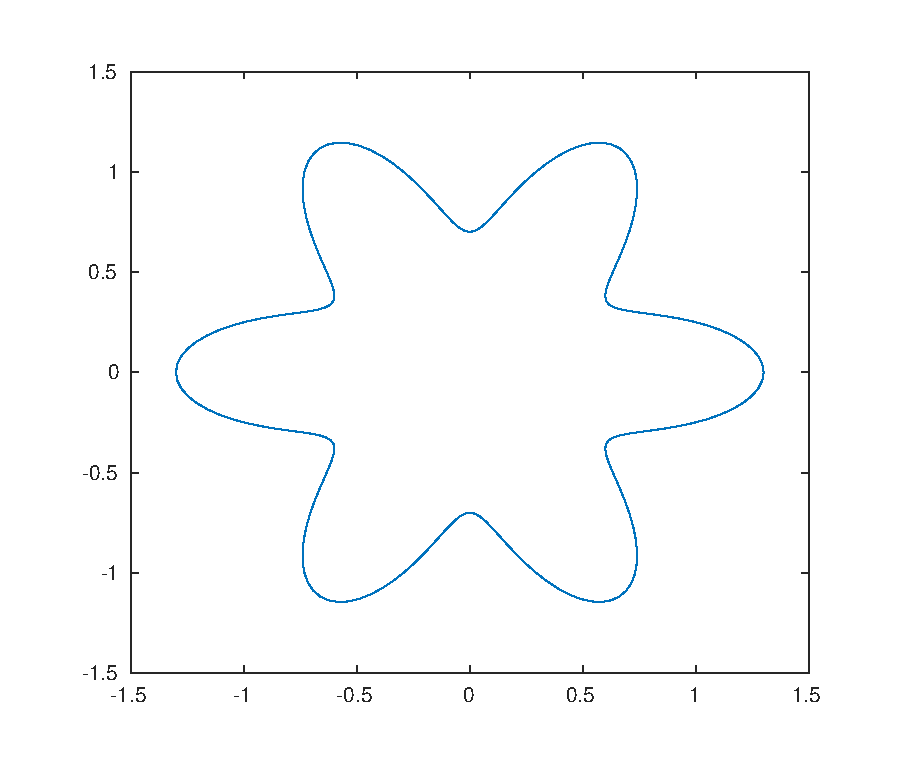
\includegraphics[width=6cm]{star.eps}                                           
  \caption{星型线}                        
\end{figure}

取终止时间$t_e=0.1$,此时曲线变化成半径为$\sqrt{209/200}$,圆心位于原点
的正圆。
\newpage
下面使用四阶隐式积分方法 ESDIRK 进行测试。误差与CPU时间的测试结果如表
\ref{tab:star1}所示,所用误差范数$\|\mathrm{E}\|_1$是用计算出的三次样
条曲线和用准确解正圆上的点生成的三次样条曲线求内部区域间近似异或面积得
出的。
\begin{table}[htbp]
    \centering\begin{tabular}{c|ccc}
        \hline
         $n$&32&ratio&64\\
                \hline
         $k$&1e-6&&5e-7\\
        \hline
        $\|\mathrm{E}\|_1$&4.49e-2&5.33&1.11e-3\\
        \hline
        CPU time(s)&2.59e+2&2.54&1.50e+3\\
        \hline
      \end{tabular}
    \caption{星型线测例: ESDIRK,终止时间$t_e = 0.1$, $h_L=4\pi/n$,$r_{\text{tiny}}=0.1$,
      $\text{Order} = 4$}
    \label{tab:star1}
  \end{table}\\
  
  中间步的计算结果图如图\ref{fig:starmidstep}所示。
  \newpage
\begin{figure}[H]
	\centering  %图片全局居中
	\subfigure[$t=0$]{
		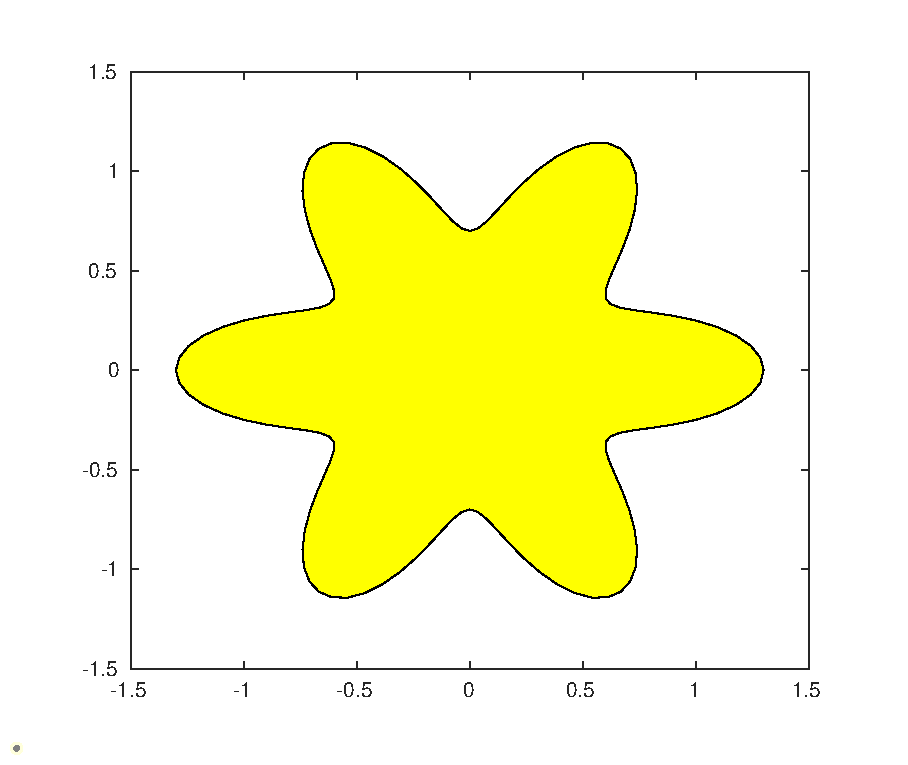
\includegraphics[width=0.3\linewidth]{star_originfill.eps}
    }
	\subfigure[$t=0.0005$]{
		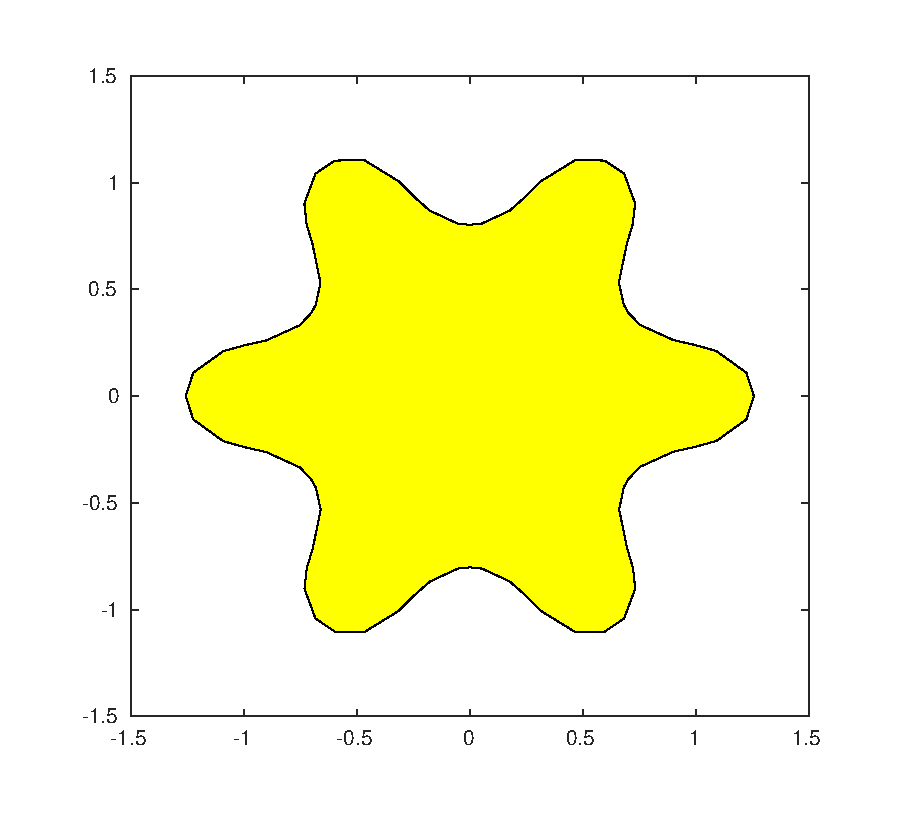
\includegraphics[width=0.3\linewidth]{star_ESDIRK64_0.0005.eps}
    }
    \subfigure[$t=0.001$]{
        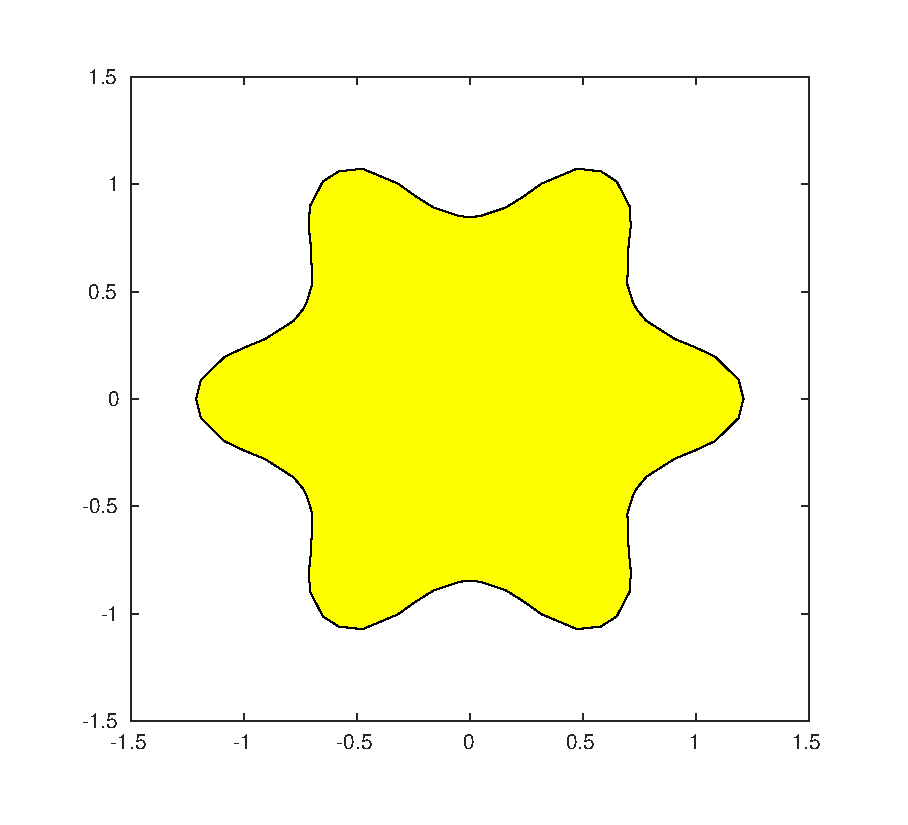
\includegraphics[width=0.3\linewidth]{star_ESDIRK64_0.001.eps}
    }\\
    \subfigure[$t=0.0015$]{
		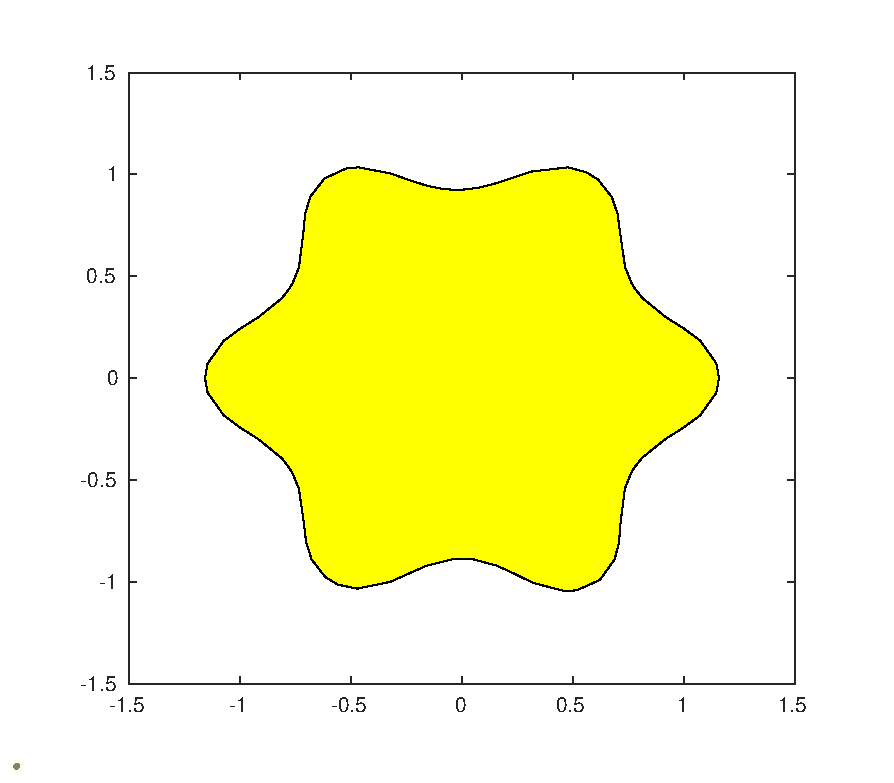
\includegraphics[width=0.3\linewidth]{star_ESDIRK64_0.0015.eps}
    }
	\subfigure[$t=0.002$]{
		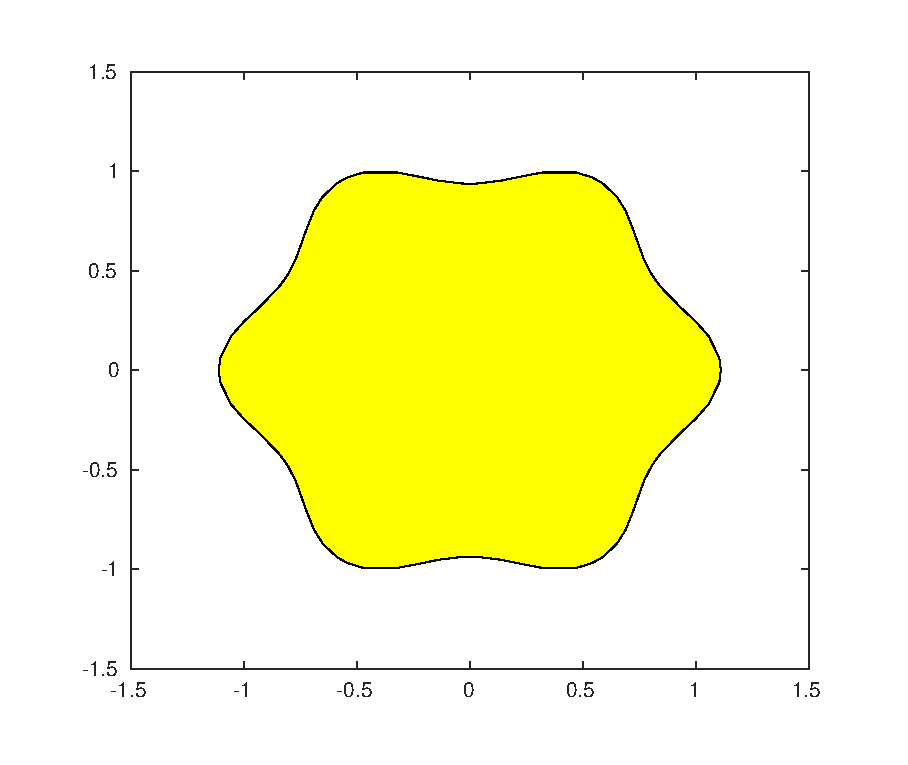
\includegraphics[width=0.3\linewidth]{star_ESDIRK64_0.002.eps}
    }
    \subfigure[$t=0.003$]{
        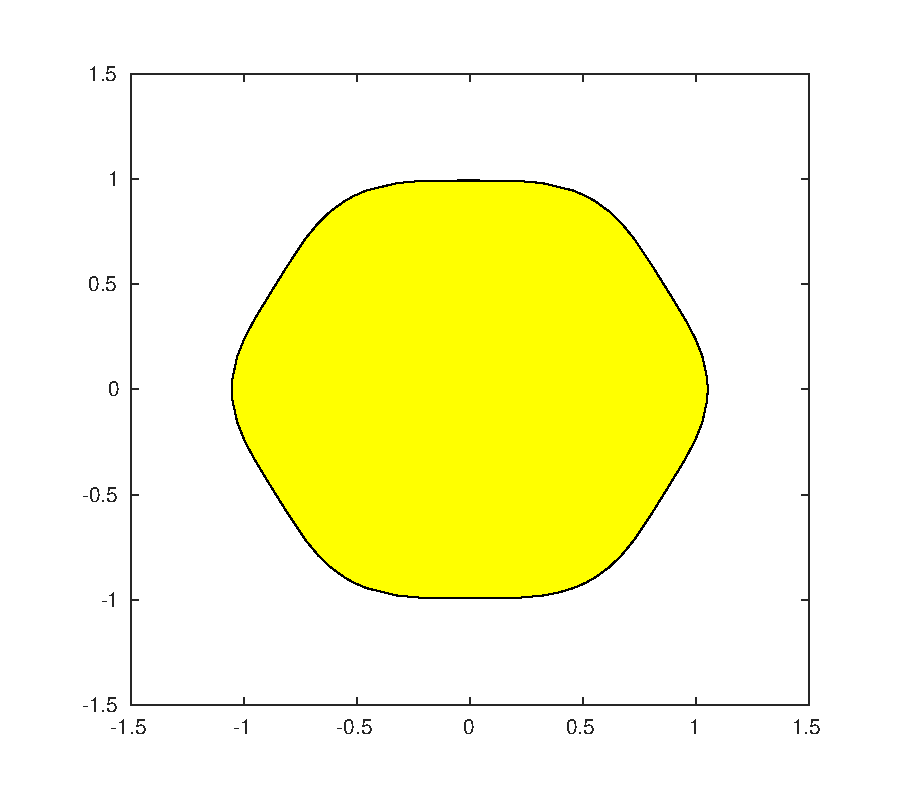
\includegraphics[width=0.3\linewidth]{star_ESDIRK64_0.003.eps}
    }\\
    \subfigure[$t=0.004$]{
		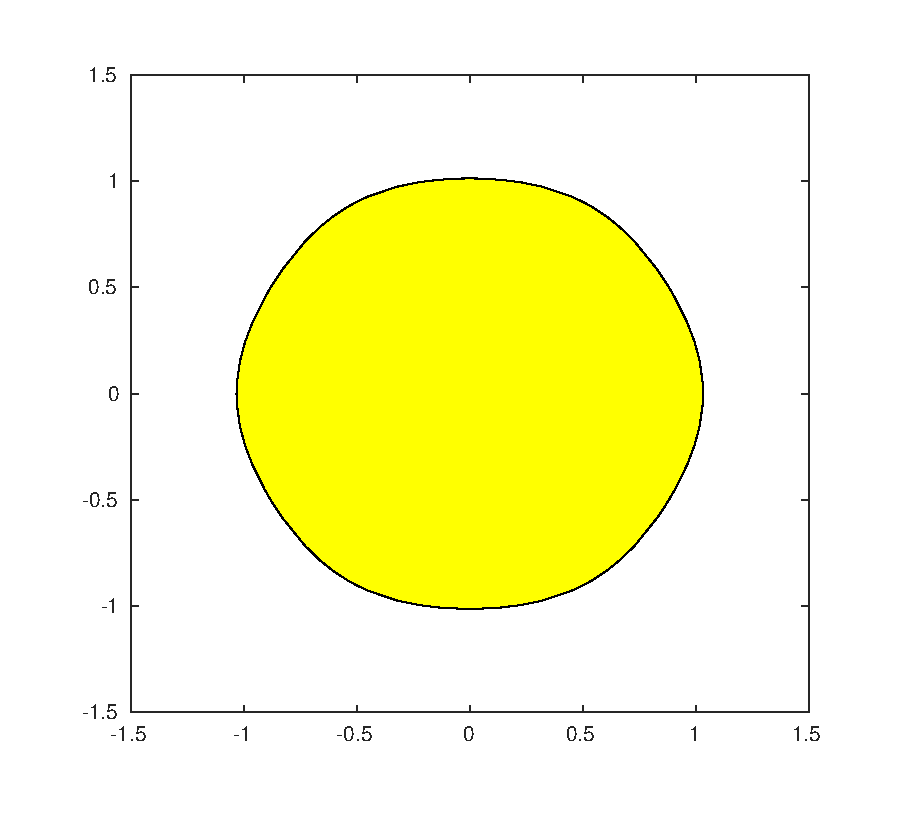
\includegraphics[width=0.3\linewidth]{star_ESDIRK64_0.004.eps}
    }
	\subfigure[$t=0.006$]{
		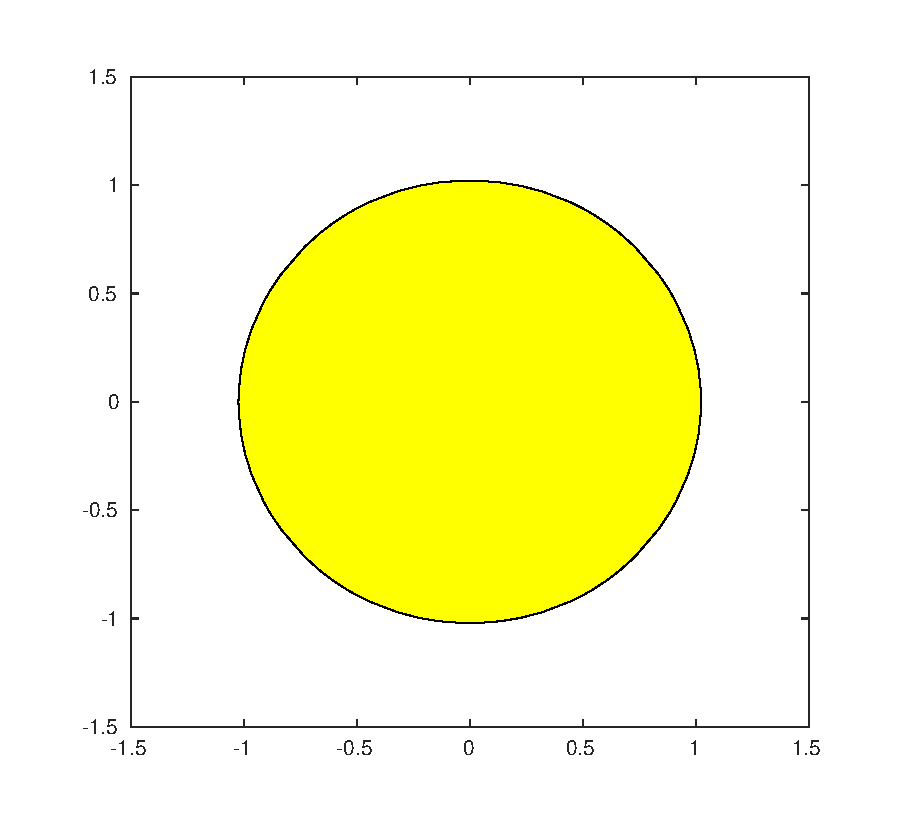
\includegraphics[width=0.3\linewidth]{star_ESDIRK64_0.006.eps}
    }
    \subfigure[$t=0.01$]{
        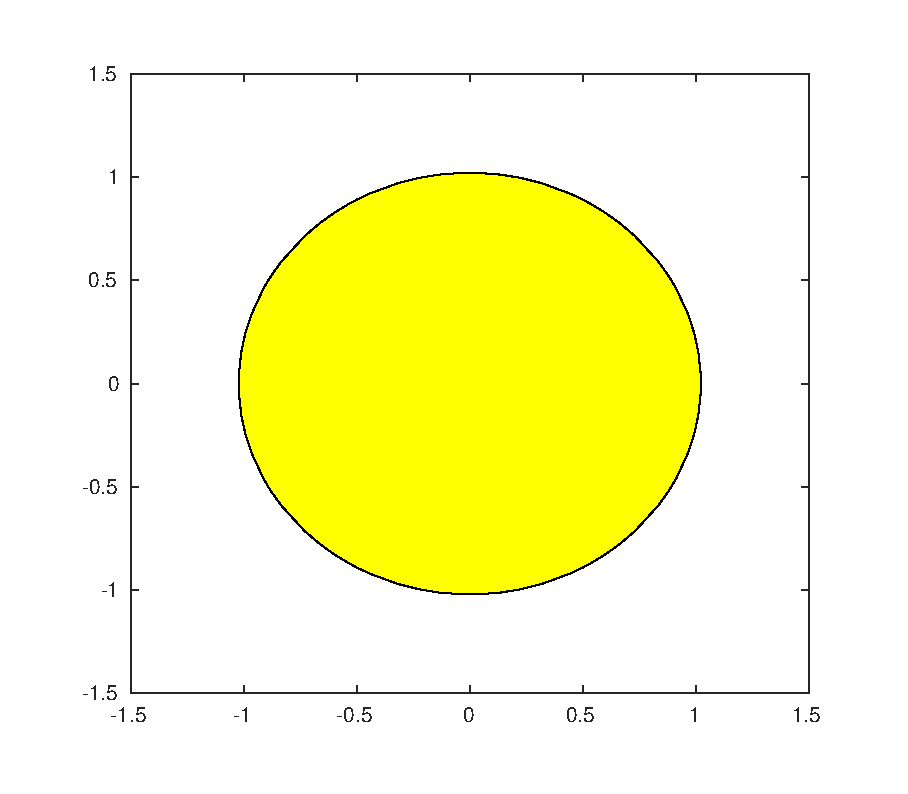
\includegraphics[width=0.3\linewidth]{star_ESDIRK64_0.01.eps}
    }
    \caption{星型线测例: 中间步计算结果图,所用参数为 $n=64$,$k=$ 1e-6,$r_\mathrm{tiny}=0.01$。}
    \label{fig:starmidstep}
\end{figure}



\end{document}
